\section{Software Allocation Problem}\label{sec_allocation}
In this section, we show our ILP model and the software-to-hardware allocation of a fault-tolerant application on heterogeneous nodes. Equation (\ref{eqn_const_func}) defines the objective function for power consumption, with constraints on timing (\ref{lbl_deadline_constraint}) (\ref{lbl_e2e_constraint}) and application reliability (\ref{lbl_reliability_constraint}). 
\begin{align}
\label{eqn_const_func}
\min_{x\in X} P(x) \\
\text{Subjected to:}\nonumber\\
\label{lbl_deadline_constraint} 
ResponseTime(x) \leq \mathrm{Deadline}\\ 
\label{lbl_e2e_constraint}
Delay(x) \leq \mathrm{E2eReq} \\
\label{lbl_reliability_constraint}
Reliability(x) \leq \mathrm{RelReq}
\end{align}

The timing constraints consist of meeting the individual tasks deadlines $Deadline$  as well as the end-to-end timing requirements of cause-effect chains $\mathrm{E2eReq}$ (\ref{lbl_e2e_constraint}) in the distributed system. The reliability constraint ensures that a feasible solution meets the application reliability requirement $\mathrm{RelReq}$. The decision variable $x$ is a 3-dimensional binary matrix that represents a feasible solution, where $x^k_{ij}$ refers to the allocation of a software component $c^k_i$ on node $m_j$ and $c^k$ refers to the $k^{th}$ replica of $c$, and $X$ is the search space of the allocation. 

In order to demonstrate our ILP optimization, we use a  simple example throughout the section which consist of software application and platform specifications: the software application is constructed from the set of components $C=\{c_1, c_2, c_3, c_4, c_5\}$, with maximum number of replicas $K=2$. The application is deployed on one or more nodes $M=\{m_1,m_2,m_3\}$. A detailed specification of the components and the nodes are shown in Table \ref{tbl_comps_config} and \ref{tbl_nodes_config}, respectively. A feasible solution $x$ to the problem is shown in Figure \ref{fig_nodes_config_feasible_solution}.
% Please add the following required packages to your document preamble:
% \usepackage{booktabs}
\begin{table}[h]
\centering
\begin{tabular}{@{}p{0.25cm}l@{}}
\toprule
C  & $R=[\text{ execution time}-(e_{m1}, e_{m2}, e_{m3}), period]$ \\ \midrule
\multirow{2}{4em}{c1} 
& [(0.030, 0.060, 0.090), 1], [(0.041, 0.081, 0.122), 2]\\[0.3em]
&[(0.083, 0.167, 0.250), 5], [(0.310, 0.620, 0.930), 10] \\[0.6em]
\multirow{2}{4em}{c2} 
& [(0.310, 0.620, 0.930), 10], [(0.310, 0.620, 0.930) 10]\\[0.3em]
&[(0.310, 0.620, 0.930), 10], [(0.310, 0.620, 0.930), 10]  \\[0.6em]
\multirow{2}{4em}{c3} 
& [(0.310, 0.620, 0.930), 10], [(0.291, 0.583, 0.874), 20]\\[0.3em]
& [(0.291, 0.583, 0.874), 20], [(0.291, 0.583, 0.874), 20]\\[0.6em]
\multirow{2}{4em}{c4} 
& [(0.291, 0.583, 0.874), 20], [(0.291, 0.583, 0.874), 20]\\[0.3em]
& [(0.291, 0.583, 0.874), 20], [(0.093, 0.186, 0.279), 50]\\[0.6em]
\multirow{2}{4em}{c5}  
& [(0.420, 0.841, 1.261), 100], [(0.420, 0.841, 1.261), 100]\\[0.3em]
& [(0.420, 0.841, 1.261), 100], [(0.420, 0.841, 1.261), 100]\\[0.3em]
\bottomrule
\end{tabular}
\caption{Timing Specification of Components and Runnables}
\label{tbl_comps_config}
\end{table}

% \begin{table}[]
% \centering
% \caption{My caption}
% \label{my-label}
% \begin{tabular}{ll}
% \hline
% M  & {[}Pmin, Pmax, lambda{]} \\ \hline
% m1 & {[}50.0,140.0,1.0E-3{]}  \\
% m2 & {[}10.0,100.0,1.0E-4{]}  \\
% m3 & {[}10.0,140.0,1.0E-5{]}  \\\hline
% \end{tabular}
% \end{table}

\begin{figure}%
\centering\small
\begin{subfigure}[b]{0.2\textwidth}
\begin{tabular}{@{}ll@{}}
\toprule
M  & {[}$P_{idle}$, $P_{max}$, $\lambda${]} \\ \midrule
$m_1$ & {[}50.0, 140.0, 1.0E-3{]}  \\
$m_2$ & {[}10.0, 100.0, 1.0E-4{]}  \\
$m_3$ & {[}10.0, 140.0, 1 .0E-5{]}  \\ \bottomrule
\end{tabular}
\captionof{figure}{Specification of Nodes}
\label{tbl_nodes_config}
\end{subfigure}~
\begin{subfigure}[b]{0.28\textwidth}
\centering
\begin{minipage}{.5\textwidth}
\raggedright
\caption*{$x^{1}$}\vspace{-0.4cm}
 $$
\begin{pmatrix} 
0 & 1 & 0\\
1 & 0 & 0\\
0 & 1 & 0\\
0 & 1 & 0\\
0 & 1 & 0
\end{pmatrix}
$$
\end{minipage}% 
~\hspace{-0.8cm}
\begin{minipage}{0.45\textwidth}
\centering
\caption*{$x^{2}$}\vspace{-0.4cm}
$$
\begin{pmatrix} 
0 & 0 & 1\\
0 & 1 & 0\\
0 & 0 & 1\\
0 & 0 & 1\\
0 & 0 & 1
\end{pmatrix}
$$
\end{minipage}
\captionof{figure}{A 3-dim. Feasible Solution, K=2}
\label{matrix_feasible_solution}
\end{subfigure}
\captionof{figure}{Example: nodes configuration, and a 3-dimensional Matrix that Represents a Feasible Solution $x$ for K=2}
\label{fig_nodes_config_feasible_solution}
\end{figure}

In the subsequent subsections, we explain the Integer Linear model, including the objective function and the constraints.

\subsection{Power Consumption Optimization }
The ILP model of the objective function is shown in (\ref{eqn_avgpowerconsumption_util}-\ref{eqn_util_component}). For a feasible solution $x$, the power consumption $P_{total}(x)$ is computed as the sum of the average power consumption of individual nodes $P_m(x)$. In order to compute the average power consumption of a node, first the node utilization is calculated using (\ref{lbl_util}), which is the sum of the components' utilization (including replicas) that are allocated to that node. A component's utilization is obtained from the sum of tasks utilization that realize the component's functionalities as shown in (\ref{eqn_util_component}).

\begin{align}
\label{eqn_avgpowerconsumption_util}
P_{total}(x) = \sum{p_{m_j}(x)}\\
\label{lbl_power}
p_{m_j}(x) = p(u_{m_j}{(x)})\\
\label{lbl_util}
u_{m_j}{(x)} = \sum_k{\sum_i{u_{c_i}*x^k_{ij}}}\\
\label{eqn_util_component}
u_c = \sum_{\tau\in T_{c}} \frac{Exec(\tau_{m_j})}{Period(\tau)}
\end{align}

Using the example, Table \ref{tbl_powerconsumption} illustrates the power consumption calculation for the feasible solution (\ref{matrix_feasible_solution}).

% In order to discriminate a feasible solution that results some nodes with highly over loaded utilization, we introduce a load-balance constraint with a maximum standard deviation $\delta^{max}$ from the expected power consumption $E(Z)$, where $Z$ is a random variable .
% \begin{align}
% \label{eqn_energyobj}
% \delta=\sqrt[]{E[Z^2]-(E[Z])^2} \leq \delta^{max}
% \end{align}

% Please add the following required packages to your document preamble:
% \usepackage{booktabs}
\begin{table}[h]
\linespread{1.0}\small
\centering
\begin{tabular}{@{}llll@{}}
\toprule
M  & C                             					& $U_c (x)$                                    & $P_m (x)$      \\ \midrule
$m_1$ & {[}$c^1_2${]}                     			& {[}0.046, 0.017{]}                       & 61.155W  \\[0.3em]
$m_2$ & {[}$c^1_1, c^2_2, c^1_3, c^1_4, c^1_5${]} 	& {[}0.196, 0.248, 0.149, & 114.648W \\[0.3em]
		& & 0.091, 0.034{]} &\\[0.3em]
$m_3$ & {[}$c^2_1, c^2_3, c^2_4, c^2_5${]}     		& {[}0.224, 0.137, 0.050{]}                & 131.731W \\[0.3em] \bottomrule
& & Total Power Consumption & 307.534W\\
\end{tabular}
\caption{Average and Total Power Consumption of Nodes}
\label{tbl_powerconsumption}
\end{table}

In the ideal case, the minimum power consumption of the distributed system is achieved by centralizing the application on fewer nodes. However, due to the timing and reliability constraints, which require additional computing resources, the optimal solution could result more used nodes. 

\subsection{Software Application Reliability}
An optimal solution $x$ must fulfill the application reliability requirement RelReq, which is usually in the range [$0.999, 0.999999$] for safety-critical applications. The ILP formulation of the application reliability constraint is shown in (\ref{eqn_appreliability_milp}), which is computed according to (\ref{eqn_appreliability}) as the total probability that the application functions over the enumerated states of the nodes, $P\!S$ that are functioning.
\begin{align}
\label{eqn_appreliability_milp}
Reliability(x)=\sum_{s\in PS}[f(x,s)]*p_s
\end{align}

, where $[f(x,s)]$ is an \textit{Iverson function } that returns $0$ if the proposition that the application functions in state $s$ is \textit{true}. Otherwise it returns $1$ if the proposition that application functions in state $s$ is \textit{false} (or the application fails in state $s$ is \textit{true}). The application functions only if all of its constituent software components functions and fails if at least of one of its components fails, which is formulated in (\ref{eqn_appreliability_milp_components}). A component functions if there exists at least one node $m_j$ that hosts the component $x_{ij}=1$ functions $s_{j}=1$, formulated in (\ref{eqn_appreliability_milp_component}). 
\begin{align}
f(x,s) = \floor[\Bigg]{\frac{\sum_if_{c_i}(x,s)}{N}}=
\begin{cases}
1 & \mbox{if } application \mbox{ functions}\\
0 & \mbox{if } application \mbox{ fails}
\end{cases}\label{eqn_appreliability_milp_components}\\
f_{c_i}(x,s) = \ceil[\Bigg]{\frac{\sum_k\sum_j x^{k}_{ij}*s_j}{K}}=
\begin{cases}
1 & \mbox{if } c_i \mbox{ functions}\\
0 & \mbox{if } c_i \mbox{ fails}
\end{cases}\label{eqn_appreliability_milp_component}
\end{align}

Table \ref{tbl_application_rel} demonstrates the application reliability calculation for the feasible solution $x$ (\ref{matrix_feasible_solution}). Figure~\ref{fig_comp_replications} shows pictorial descriptions of component allocations on nodes with no replication $K=1$, and with replications $K=2$. 
\begin{table}[h]
\centering
\begin{tabular}{@{}llll@{}}
\toprule
$s$   & $p_s$     & {[}$f_{c_i}(x), i=1,2,3,4${]} & $f_a(x)$ \\ \midrule
000 & 0.0000000000 & {[}0, 0, 0, 0{]}          & 0     \\
001 & 0.0000000099 & {[}0, 0, 0, 1{]}          & 0     \\
010 & 0.0000000099 & {[}1, 1, 1, 1{]}          & 1     \\
011 & 0.0000999800 & {[}1, 1, 1, 1{]}          & 1     \\
100 & 0.0000000099 & {[}1, 1, 1, 0{]}          & 0     \\
101 & 0.0000999800 & {[}1, 1, 1, 0{]}          & 0     \\
110 & 0.0000999800 & {[}1, 1, 1, 1{]}          & 1     \\
111 & 0.9997000299 & {[}1, 1, 1, 1{]}          & 1     \\ \bottomrule
\end{tabular}
\caption{Application reliability calculation using state enumeration method, R(x) = 0.9998999998.}
\label{tbl_application_rel}
\end{table}

\begin{figure}
    \centering
    \begin{subfigure}[b]{0.2\textwidth}
        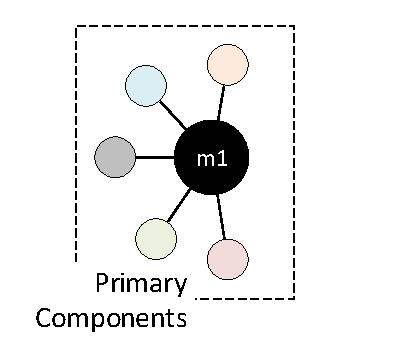
\includegraphics[width=\textwidth]{k0}
        \caption{No replication, K = 1.}
        \label{fig:datachainsingle}
    \end{subfigure}
    ~ %add desired spacing between images, e. g. ~, \quad, \qquad, \hfill etc. 
      %(or a blank line to force the subfigure onto a new line)
    \begin{subfigure}[b]{0.25\textwidth}
        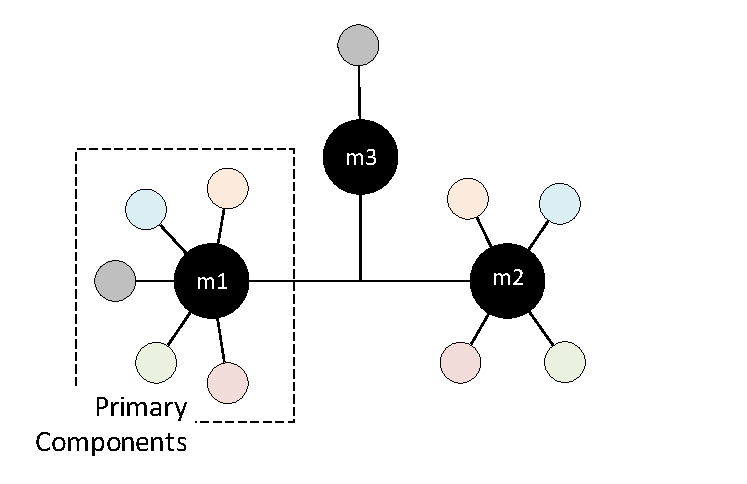
\includegraphics[width=\textwidth]{k1}
        \caption{With replication, K = 2.}
        \label{fig:datachainmulti}
    \end{subfigure}
%     ~
%         \begin{subfigure}[b]{0.3\textwidth}
%         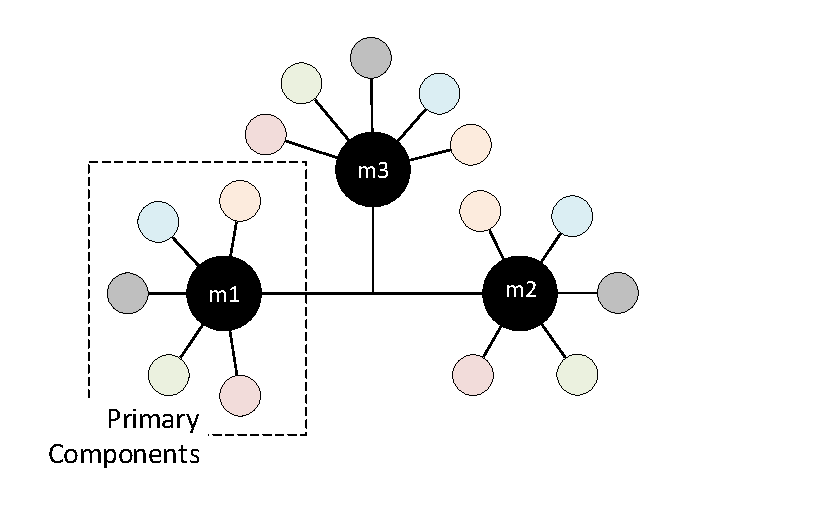
\includegraphics[width=\textwidth]{k2}
%         \caption{With Replication, K = 3}
%         \label{fig:datachainsingle}
%     \end{subfigure}
    \caption{Allocation of components.}
    \label{fig_comp_replications}
\end{figure}

In the case that the application reliability could be met with less replications, there is no need to keep unnecessary component replicas in the system. To this end, the optimization algorithm imposes soft constraints for $k>1$, which implies replicas can be allocated with \textit{overlapping}, that is, the same components can be allocated on the same node. In this case, redundant components should be discarded by design since the reliability does not improve as a result of additional replicas on the same node.

\subsection{Timing Constraints}
The timing constraints ensure that the response times of the tasks realizing the distributed application meet their deadlines. Furthermore, they ensure that the cause-effect chains satisfy their respective end-to-end timing requirements, for all possible failure-modes of the system. The constraints are formulated as logical constraints in the ILP problem, as explained in the rest of this subsection.

\subsubsection*{Tasks Deadline Constraints}
The following pseudo-code illustrates how the ILP logical constraints of the tasks deadlines are prepared. It explores all possible set of components combinations (or partitions) that can potentially be allocated to a node. And only the sets that are schedulable are asserted as constraints in to the optimization problem, which is explained as follows: Line (1) identifies the power set of the components $Par$, followed by synthesis of tasks models of each partition. Line (2) checks the tasks models' schedulability and returns a matrix $M^T$ that indicate schedulability, which is \textit{true} if the task model is schedulable and \textit{false} if not schedulable. Line (3) generates an ILP partition expression $E$ for each node, then Line (4-6) asserts the expressions to hold in the optimization for the partitions that are schedulable.
\begin{algorithm}
\caption{Generate task partitions constraints.}\label{alg_partition}
% \algsetup{
% linenosize=\small,
% linenodelimiter=.
% }	
\renewcommand{\algorithmicrequire}{\textbf{Input:}}
%\renewcommand{\algorithmicensure}{\textbf{Output:}}
\begin{algorithmic}[1]
\Require $C,M$
\Ensure Optimization Satisfies Tasks Deadlines, $D$
\State $Par \Leftarrow 2^C$	
\State $M^T\Leftarrow isSched(Par, M)$
\State $E\Leftarrow MilpParExp(x)$
\ForAll{$m \in M$}
	\State $assertOR(M^T_m, E_m, true)$
\EndFor
\end{algorithmic}
\end{algorithm}

In general, the number of potential logical constraints grow exponentially, which is in $2^{|C|}*|M|$. However, the effective logical constraints that are eventually asserted are much lower, for two main reasons: 1) a portion of the tasks models are not schedulable, therefore eliminated from the power set, due to CPU utilization exceeding the bound, not satisfying response time of either task in the partition; ii) a task model can be a super set of other tasks model. In this case, only the super model is checked, hence reducing pre-optimization time and logical constraints asserted in the solver.

\subsubsection*{Cause-effect Chains Constraints}
These constraints ensure that the cause-effect chains $\Gamma$ meet their respective end-to-end requirements $\mathrm{E2eReq}$. Similar to the previous constraints, the cause-effect chain constraints are logical assertions, which must be fulfilled by the optimal solution. The following pseudo-code illustrates how the ILP logical assertions are synthesized from the input models. 

% A cause-effect chain may consist of two or more tasks, and depending on the eventual allocation of the tasks to nodes, the chain could be hosted on a standalone node, distributed across multiple nodes. 
The pseudo-code contains three main parts: i) the first part in Line (2) identifies the different deployment cases of the cause-effect chains over a set of nodes $M$; ii) the second part in Line (3-5), checks the schedulability of a deployable cause-effect chain $\phi$ against the Reaction or Age delays  \cite{mubeen2013support} and returns its schedulability matrix $M^\Gamma$, with values $true$ if schedulable and $false$ if not schedulable. For a schedulable $\phi$, Line (5) constructs a conjunctive ILP expression that indicates the existence of at least one schedulable $\phi$ that satisfies the end-to-end requirement imposed on $\gamma$; iii) the last part in Line (7) asserts the ILP logical OR expressions for each $\gamma$.
\begin{algorithm}
\caption{Generate constraints on the cause-effect chains.}\label{alg_causeeffectchains}
\begin{algorithmic}[1]
\Require $\Gamma,M$
\Ensure Optimization Satisfies End-to-end Requirements of Cause-effect Chains
\ForAll{$\gamma \in \Gamma$}
\State $\Phi\leftarrow Unique(C^{T_\Gamma}_r, M)$ 
	\ForAll{$\phi \in \Phi$}
    \State $M^\Gamma\Leftarrow isSched(\phi, M)$
    \State $depExp\Leftarrow depExp \lor sched(M^\Gamma, true)$
    \EndFor
	\State $assert(depExp)$
\EndFor
\end{algorithmic}
\end{algorithm}

